%!TEX root = ../dissertation.tex
\begin{savequote}[75mm]
This is some random quote to start off the chapter.
\qauthor{Firstname lastname}
\end{savequote}

\hypertarget{(chap:inquadramento)}{}
\chapter{Inquadramento delle attività di stage}

\section{Il progetto aziendale}
Per riuscire ad inquadrare al meglio lo scopo del progetto di stage è importante capire a fondo il progetto generale che l'azienda porta avanti da ormai alcuni anni, poiché essi sono tra loro intrinsecamente legati. Il progetto generale mira a fornire un prodotto che possa far progredire il mercato del trasporto attraverso la digitalizzazione dello stesso, questo attraverso il superamento dei vecchi gestionali, utilizzati concretamente solo per la fatturazione, e l'introduzione di una piattaforma web attraverso cui gestire ogni passaggio nel rapporto cliente-operatore.
Il software permette di gestire la flotta di mezzi e organizzare gli ordini di carico e scarico commissionati dai clienti, questa organizzazione può essere fatta manualmente da un operatore esperto oppure affidandosi ad algoritmi che organizzino gli ordini utilizzando i camion disponibili nel miglior modo possibile. Il sistema dispone di un algortimo per il \glo{vehicle routing}, su cui si può dire faccia capo l'intero progetto, questo si occupa di ottimizzare i viaggi dei camionisti tenendo conto di un numero incredibile di variabili, questo algoritmo ha subito diverse upgrade in un'ottica di miglioramento continuo, per renderlo più efficiente, più versatile e più preciso.
In questo contesto l'euristica che fornisce la valutazione approssimativa dello spazio occupato da un certo numero di merci è molto importante, questo perché è necessario sapere quanti mezzi siano necessari per trasportare le merci richieste e quanto spazio sia ancora disponibile per ordini futuri.

\section{Il progetto di stage}
Il progetto di stage dopo l'evento \glo{StageIt} ed alcune riunione presso l'azienda è stato studiato dettagliatamente e riportato nel documento piano di lavoro, nello stesso sono riportati gli obiettivi e la pianificazione delle attività.
L'importanza di ottenere una valutazione reale dello spazio occupato da un certo numero di oggetti è fondamentale, per fare ciò lo stage prevede la realizzazione di diversi modelli, lo sviluppo di tali modelli sarà incrementale in quanto ciascun modello eredita quanto sviluppato nel precedente. Ogni modello per definizione permetterà di individuare la disposizione ottima dell'\glo{istanza} corrente, questa potrà poi essere confrontata con quella fornita dall'euristica, da questo confronto potremo individuare informazioni utili che permettano di valutare oggettivamente la bontà delle soluzioni fornite dall'euristica, questo permette di capire se con il passare delle versioni rilasciate l'euristica sta migliorando e di quanto rispetto al passato.

\section{Problema del bin packing}
Il problema sopra riportato può essere approssimato considerando il container del camion e merc
Il problema del Bin Packing è uno dei problemi più studiati nell'ambito della ricerca operativa, dato un insieme I = \{1,...,n\} di parallelepipedi aventi dimensioni $w_{i}$, $d_{i}$ e $h_{i}$ con i $\in$ I, ciascuno di questi  l'obiettivo è quello di utilizzare il minor numero di contenitori di uguali dimensioni W e D che riescano a contenere tutti gli oggetti dell'insieme I.\\
\begin{figure}[!h]
    \begin{center} 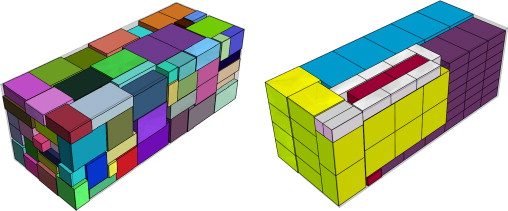
\includegraphics[scale=1]{figures/bin_packing}
        \caption[ciucia]{Ciclo di vita documentazione}
        \label{fig:myInlineFigure}
    \end{center}
\end{figure}
\newline
In realtà siamo interessati ad una variante del sopra citato problema, quella dello Strip Packing, dove la lunghezza del contenitore è infinita e si deve disporre l'insieme N di oggetti nel modo migliore affinché si minimizzi la lunghezza lineare occupata dagli oggetti.
